\documentclass[aspectratio=169,10pt]{beamer}

% ---------- 中文与字体 ----------
\usepackage{fontspec}
\usepackage{xeCJK}
\setmainfont{DejaVu Sans}
\setsansfont{DejaVu Sans}
\setCJKmainfont{Noto Sans CJK SC}
\setCJKsansfont{Noto Sans CJK SC}
\setCJKmonofont{Noto Sans Mono CJK SC}

% ---------- Packages ----------
\usepackage{amsmath,amssymb}
\usepackage{booktabs}
\usepackage{array}
\usepackage{graphicx}
\usepackage{xcolor}
\usepackage{hyperref}
\usepackage{tikz}
\usetikzlibrary{arrows.meta,positioning,calc,decorations.pathreplacing}

% ---------- Theme ----------
\usetheme{Madrid}
\usefonttheme{professionalfonts}
\setbeamertemplate{navigation symbols}{}
\setbeamertemplate{footline}[frame number]
\setbeamertemplate{caption}[numbered]

\definecolor{BioBlue}{HTML}{0B3558}
\definecolor{BioTeal}{HTML}{0E8C86}
\definecolor{BioGreen}{HTML}{38A169}
\definecolor{BioOrange}{HTML}{F59E0B}
\definecolor{BioRed}{HTML}{E53E3E}
\definecolor{BioGray}{HTML}{F4F7FA}
\definecolor{TextGray}{HTML}{2D3748}
\definecolor{LightBlue}{HTML}{E6F2FF}
\definecolor{LightTeal}{HTML}{E6FFFA}

\setbeamercolor{palette primary}{bg=BioBlue,fg=white}
\setbeamercolor{palette secondary}{bg=BioTeal,fg=white}
\setbeamercolor{frametitle}{bg=BioBlue,fg=white}
\setbeamercolor{title}{fg=white,bg=BioBlue}
\setbeamercolor{block title}{bg=BioBlue,fg=white}
\setbeamercolor{block body}{bg=BioGray,fg=TextGray}
\setbeamercolor{alerted text}{fg=BioRed}
\setbeamercolor{normal text}{fg=TextGray,bg=white}

\graphicspath{{./}{/mnt/data/}}
\hypersetup{colorlinks=true,linkcolor=BioBlue,urlcolor=BioTeal}

% ---------- Helpers ----------
\newcommand{\chip}[2]{\tikz[baseline=(x.base)]\node[rounded corners=2pt,fill=#1!15,draw=#1!70,inner xsep=5pt,inner ysep=2pt](x){\scriptsize\textbf{#2}};}
\newcommand{\key}[1]{\textbf{\textcolor{BioTeal}{#1}}}
\newcommand{\metric}[2]{\textbf{#1}\;{\textcolor{BioGreen}{\footnotesize #2}}}

\title[BioRAG 中文版]{BioRAG：让医学问答系统查得更准、答得更稳}
\subtitle{对比学习微调 + Cross-Encoder 二次筛选}
\author{Group 2}
\institute{BioASQ 12b Project Presentation}
\date{\today}

\begin{document}

% 1
\begin{frame}
  \titlepage
  \vspace{-0.4em}
  \begin{center}
    \chip{BioBlue}{医学问答} \hspace{0.4em}
    \chip{BioTeal}{RAG} \hspace{0.4em}
    \chip{BioOrange}{InfoNCE} \hspace{0.4em}
    \chip{BioGreen}{重排序}
  \end{center}
\end{frame}

% 2
\begin{frame}{一句话介绍：我们在解决什么问题？}
\begin{block}{普通 RAG 像“开卷考试”}
大模型不是直接凭记忆回答，而是先去查资料，再根据查到的资料生成答案。
\end{block}

\vspace{0.4em}
\begin{alertblock}{但医学问答不能“查错资料”}
医学文本里有很多专业名词、缩写和细微差别。\textbf{资料看起来相关，不代表真的能回答问题。}
\end{alertblock}

\vspace{0.4em}
\begin{center}
\Large \key{目标：}让系统\textbf{查得更准}，也\textbf{不要被错误证据带偏}。
\end{center}
\end{frame}

% 3
\begin{frame}{为什么普通 RAG 在医学领域容易出错？}
\begin{columns}[T,onlytextwidth]
\column{0.48\textwidth}
\begin{block}{问题 1：术语不一定对得上}
同一个医学概念可能有不同说法：
\vspace{0.4em}
\begin{center}
\chip{BioBlue}{myocardial infarction} \quad $\approx$ \quad \chip{BioTeal}{heart attack}
\end{center}
\vspace{0.4em}
如果模型没有学过医学语义，就可能匹配失败。
\end{block}

\column{0.48\textwidth}
\begin{block}{问题 2：表面相关可能方向相反}
有些文档关键词相似，但语义并不能支持答案。
\vspace{0.4em}
\begin{center}
\chip{BioOrange}{看起来相关} \quad $\rightarrow$ \quad \chip{BioRed}{自信答错}
\end{center}
\vspace{0.4em}
这就是 retrieval-induced hallucination。
\end{block}
\end{columns}

\vspace{0.5em}
\begin{center}
\textbf{医学问答的关键不是“有没有资料”，而是“资料靠不靠谱”。}
\end{center}
\end{frame}

% 4
\begin{frame}{BioRAG 整体流程}
\centering
\begin{tikzpicture}[
  node distance=0.55cm,
  box/.style={draw=BioBlue,rounded corners=4pt,fill=LightBlue,minimum width=2.25cm,minimum height=0.95cm,align=center,font=\small},
  proc/.style={draw=BioTeal,rounded corners=4pt,fill=LightTeal,minimum width=2.35cm,minimum height=0.95cm,align=center,font=\small},
  final/.style={draw=BioGreen,rounded corners=4pt,fill=BioGreen!12,minimum width=2.25cm,minimum height=0.95cm,align=center,font=\small},
  arrow/.style={-{Latex[length=3mm]},thick,BioBlue}
]
\node[box] (q) {医学问题};
\node[proc,right=of q] (retr) {微调后的\\检索器};
\node[proc,right=of retr] (top20) {先找出\\Top-20};
\node[proc,right=of top20] (rerank) {重排序模型\\二次筛选};
\node[final,right=of rerank] (ans) {生成\\最终答案};
\draw[arrow] (q) -- (retr);
\draw[arrow] (retr) -- (top20);
\draw[arrow] (top20) -- (rerank);
\draw[arrow] (rerank) -- (ans);
\node[below=0.55cm of retr,align=center,font=\scriptsize,text=TextGray] {先快速找资料};
\node[below=0.55cm of rerank,align=center,font=\scriptsize,text=TextGray] {再认真筛证据};
\end{tikzpicture}

\vspace{0.8em}
\begin{block}{核心思想}
\textbf{检索器负责“找得全”，重排序模型负责“筛得准”，生成模型负责“根据可靠证据回答”。}
\end{block}
\end{frame}

% 5
\begin{frame}{第一步：Baseline 怎么做？}
\begin{columns}[T,onlytextwidth]
\column{0.52\textwidth}
\begin{block}{Zero-shot Baseline}
\begin{itemize}
  \item 使用冻结的 PubMedBERT bi-encoder
  \item 把问题和文档分别变成向量
  \item 用向量相似度找 Top-3 文档
  \item 直接交给 Qwen-2.5 生成答案
\end{itemize}
\end{block}

\begin{alertblock}{优点和缺点}
优点：速度快。\quad 缺点：只看“像不像”，不一定真正理解医学语义。
\end{alertblock}

\column{0.43\textwidth}
\begin{center}
\Large
问题向量 $\rightarrow$ 文档向量\\[0.8em]
$\Downarrow$\\[0.6em]
相似度打分\\[0.8em]
$\Downarrow$\\[0.6em]
Top-3 直接生成
\end{center}
\end{columns}
\end{frame}

% 6
\begin{frame}{第二步：让检索器更懂医学}
\begin{block}{InfoNCE 可以通俗理解为“配对训练”}
给模型很多组\textbf{问题 - 正确资料}，让它学会：
\end{block}

\vspace{0.4em}
\begin{columns}[T,onlytextwidth]
\column{0.48\textwidth}
\begin{block}{正确配对}
\centering
\Large 问题 \quad $\leftrightarrow$ \quad 相关文档\\[0.4em]
\chip{BioGreen}{拉近}
\end{block}

\column{0.48\textwidth}
\begin{block}{错误配对}
\centering
\Large 问题 \quad $\nleftrightarrow$ \quad 不相关文档\\[0.4em]
\chip{BioRed}{推远}
\end{block}
\end{columns}

\vspace{0.6em}
\begin{center}
训练后，检索器不只是看关键词，而是更能理解\key{医学语义相关性}。
\end{center}
\end{frame}

% 7
\begin{frame}{第三步：加一个“审稿人”筛证据}
\begin{columns}[T,onlytextwidth]
\column{0.49\textwidth}
\begin{block}{Bi-encoder 像快速初筛}
\begin{itemize}
  \item 问题和文档分开读
  \item 速度快
  \item 但细节判断不够强
\end{itemize}
\end{block}

\column{0.49\textwidth}
\begin{block}{Cross-encoder 像认真审稿}
\begin{itemize}
  \item 把问题和文档放在一起读
  \item 能看出更细的语义关系
  \item 用来从 Top-20 中选 Top-3
\end{itemize}
\end{block}
\end{columns}

\vspace{0.6em}
\begin{alertblock}{为什么有用？}
它可以过滤掉“看起来相关、其实不能回答问题”的文档，减少错误证据进入生成模型。
\end{alertblock}
\end{frame}

% 8
\begin{frame}{实验设置}
\begin{columns}[T,onlytextwidth]
\column{0.50\textwidth}
\begin{block}{数据集}
\begin{itemize}
  \item BioASQ 12b 生物医学问答任务
  \item 抽取 500 个问题做测试
  \item 覆盖 Yes/No、Factoid、List、Summary
  \item 训练数据和测试问题不重叠
\end{itemize}
\end{block}

\column{0.46\textwidth}
\begin{block}{主要指标}
\begin{tabular}{>{\bfseries}p{0.30\linewidth}p{0.58\linewidth}}
Yes/No & Accuracy, Macro-F1 \\
Factoid & Strict Accuracy, MRR \\
List & Recall, F-measure \\
生成质量 & ROUGE-L, BERTScore \\
\end{tabular}
\end{block}

\begin{block}{训练细节}
3 个 epoch；学习率 $2\times10^{-5}$；batch size 16；最大长度 512。
\end{block}
\end{columns}
\end{frame}

% 9
\begin{frame}{训练过程：Loss 一直下降}
\begin{columns}[T,onlytextwidth]
\column{0.62\textwidth}
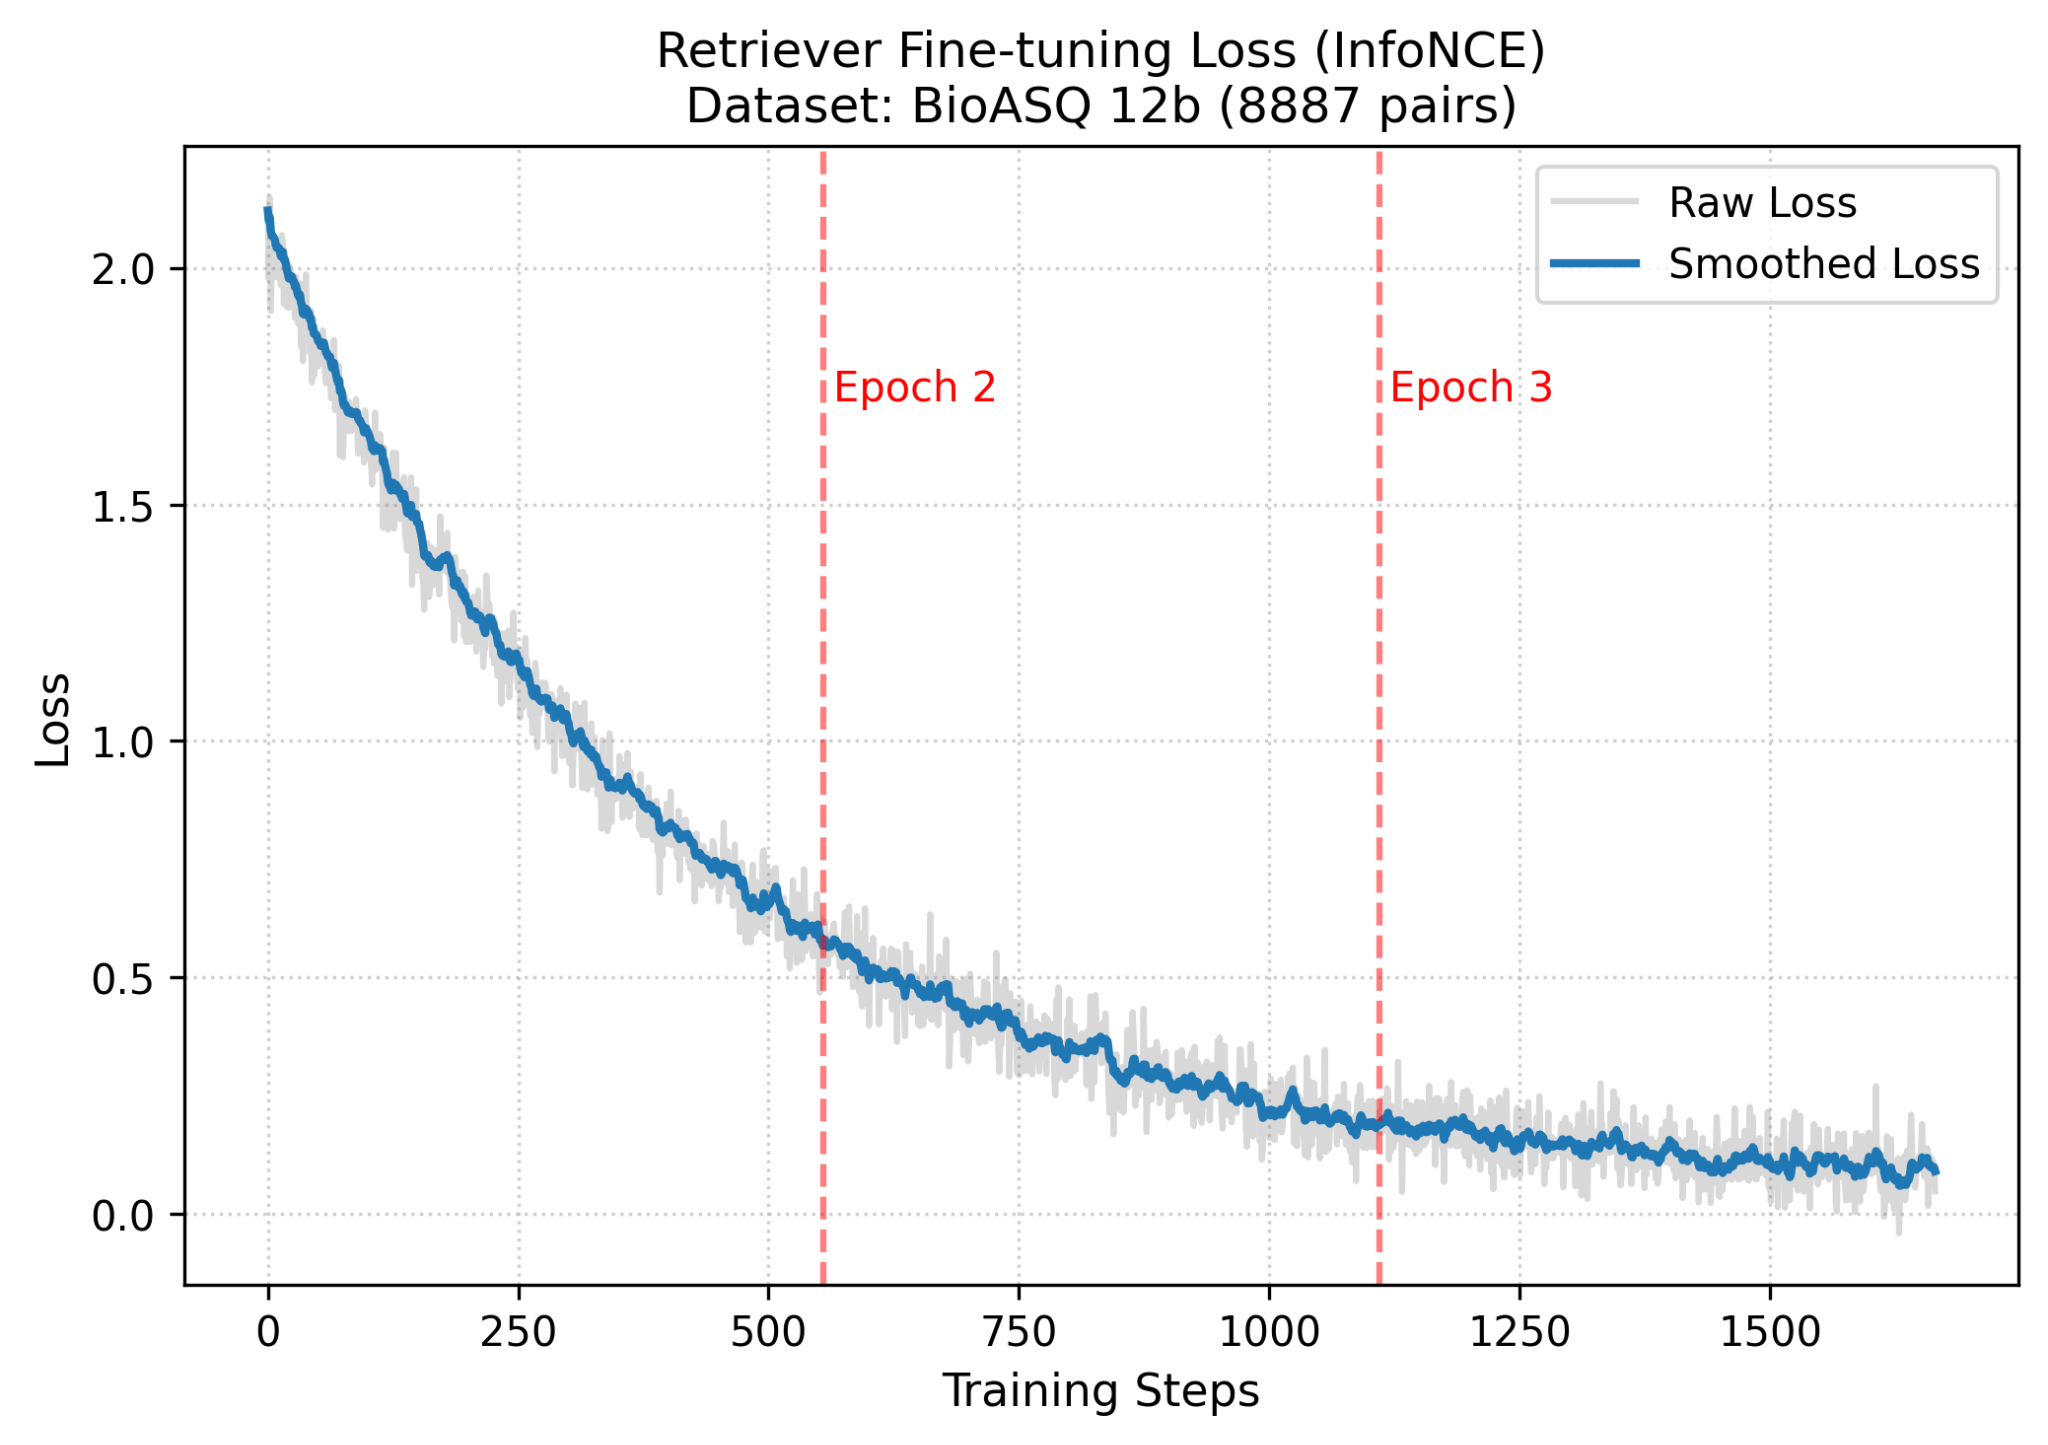
\includegraphics[width=\linewidth]{aligned_training_loss.png}

\column{0.34\textwidth}
\begin{block}{怎么读这张图？}
\begin{itemize}
  \item 一开始 loss 较高：模型还不会区分好资料和坏资料
  \item 前期快速下降：模型学得很快
  \item 后期趋于稳定：训练基本收敛
\end{itemize}
\end{block}
\begin{alertblock}{结论}
检索器学到了更适合医学问答的表示空间。
\end{alertblock}
\end{columns}
\end{frame}

% 10
\begin{frame}{实验结果：BioRAG 明显优于 Baseline}
\small
\begin{table}
\centering
\begin{tabular}{llccc}
\toprule
问题类型 & 指标 & Baseline & BioRAG & 提升 \\
\midrule
Yes/No & Accuracy & 0.6364 & \textbf{0.7692} & \textcolor{BioGreen}{+20.9\%} \\
Yes/No & Macro-F1 & 0.6137 & \textbf{0.7410} & \textcolor{BioGreen}{+20.7\%} \\
Factoid & Strict Acc. & 0.3869 & \textbf{0.4526} & \textcolor{BioGreen}{+17.0\%} \\
List & Recall & 0.3242 & \textbf{0.4133} & \textcolor{BioGreen}{+27.5\%} \\
Overall & BERTScore & 0.8643 & \textbf{0.8679} & \textcolor{BioGreen}{+0.4\%} \\
\bottomrule
\end{tabular}
\end{table}

\vspace{0.4em}
\begin{block}{重点观察}
\begin{itemize}
  \item List Recall 提升最大：说明系统更能找全多个答案
  \item Yes/No Accuracy 提升明显：说明系统更不容易被错误证据带偏
\end{itemize}
\end{block}
\end{frame}

% 11
\begin{frame}{速度权衡：慢了一点，但更可靠}
\begin{columns}[T,onlytextwidth]
\column{0.46\textwidth}
\begin{block}{平均每个问题耗时}
\begin{center}
\Large
Baseline：\textbf{2.60 秒}\\[0.6em]
BioRAG：\textbf{3.31 秒}\\[0.6em]
\chip{BioOrange}{额外 +0.71 秒}
\end{center}
\end{block}

\column{0.50\textwidth}
\begin{alertblock}{为什么会变慢？}
Cross-encoder 要认真检查 20 个候选文档，所以计算量更大。
\end{alertblock}

\begin{block}{为什么仍然值得？}
多花不到 1 秒，换来 Yes/No 和 List 问题上 20\% 左右的关键提升。医学问答里，\textbf{可靠性比快一点更重要}。
\end{block}
\end{columns}
\end{frame}

% 12
\begin{frame}{案例分析：有时候“不知道”比答错更好}
\begin{block}{问题}
\centering
\Large Does physical activity influence gut hormones?\\[0.3em]
\chip{BioGreen}{标准答案：Yes}
\end{block}

\begin{columns}[T,onlytextwidth]
\column{0.48\textwidth}
\begin{alertblock}{Baseline}
检索到一篇关于 bed rest / inactivity 的弱相关文档，结果错误地回答 \textbf{No}。
\end{alertblock}
\begin{center}
\chip{BioRed}{自信但错误}
\end{center}

\column{0.48\textwidth}
\begin{block}{BioRAG}
重排序模型过滤掉弱证据，最终回答 \textbf{I don't know}。
\end{block}
\begin{center}
\chip{BioGreen}{保守但安全}
\end{center}
\end{columns}

\vspace{0.4em}
\begin{center}
\textbf{在医学场景里，证据不足时承认不知道，通常比编造答案更安全。}
\end{center}
\end{frame}

% 13
\begin{frame}{讨论：BioRAG 到底改进了哪里？}
\begin{columns}[T,onlytextwidth]
\column{0.32\textwidth}
\begin{block}{检索器}
更懂医学语义，不只依赖表面关键词。
\end{block}

\column{0.32\textwidth}
\begin{block}{重排序器}
像“证据审稿人”，把弱相关材料筛掉。
\end{block}

\column{0.32\textwidth}
\begin{block}{生成模型}
看到更干净的上下文，所以更不容易胡说。
\end{block}
\end{columns}

\vspace{0.6em}
\begin{alertblock}{局限性}
Cross-encoder 会增加延迟；最终 LLM 还没有端到端微调；测试只用了 500 个问题，后续可以扩大规模验证。
\end{alertblock}
\end{frame}

% 14
\begin{frame}{结论}
\begin{block}{主要结论}
在医学问答中，RAG 的关键不只是“能查资料”，而是\textbf{能查到对的资料，并且不被错的资料带偏}。
\end{block}

\vspace{0.5em}
\begin{itemize}
  \item InfoNCE 微调：让 retriever 更懂医学语义
  \item Cross-encoder 重排序：过滤掉不可靠证据
  \item 实验结果：List Recall 和 Yes/No Accuracy 提升最明显
  \item 速度代价：平均只增加 0.71 秒
\end{itemize}

\vfill
\begin{center}
\Large \textbf{先对齐检索器，再验证证据，最后安全生成。}\\[0.6em]
谢谢大家！欢迎提问。
\end{center}
\end{frame}

% 15
\begin{frame}[allowframebreaks]{参考文献}
\footnotesize
\begin{thebibliography}{99}
\bibitem{bioasq12b} BioASQ. \emph{Tasks 12b, Synergy12, MultiCardioNER, BioNNE -- Year 12}. \url{https://www.bioasq.org/participate/challenges_year_12}
\bibitem{rag} Lewis et al. \emph{Retrieval-Augmented Generation for Knowledge-Intensive NLP Tasks}. NeurIPS, 2020. \url{https://arxiv.org/abs/2005.11401}
\bibitem{infonce} van den Oord, Li, and Vinyals. \emph{Representation Learning with Contrastive Predictive Coding}. arXiv:1807.03748, 2018. \url{https://arxiv.org/abs/1807.03748}
\bibitem{pubmedbert} Gu et al. \emph{Domain-Specific Language Model Pretraining for Biomedical Natural Language Processing}. ACM TCH, 2021.
\bibitem{minilm} Wang et al. \emph{MiniLM: Deep Self-Attention Distillation for Task-Agnostic Compression of Pre-trained Transformers}. NeurIPS, 2020.
\end{thebibliography}
\end{frame}

\end{document}
